% Diagrama de cuerpo libre DE EJEMPLO (bloque con F, N, W y fricción).
% Para un problema real del Banco, nombra el archivo con el ID exacto:
% DIN-001.tex -> imagenes/render/DIN-001.png (el build usa el nombre del
% archivo, sin extensión, como nombre del PNG). Ver ../../docs/IMAGENES.md.
\documentclass[tikz,border=3pt]{standalone}
\usepackage{amsmath}
\usetikzlibrary{arrows.meta}
\begin{document}
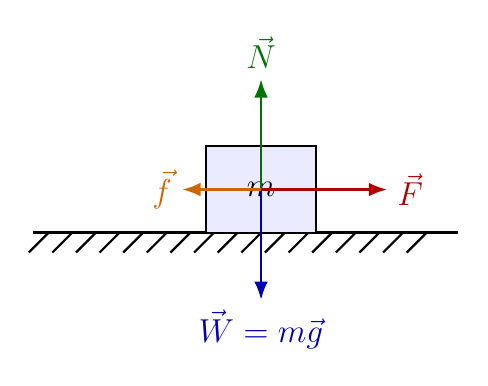
\begin{tikzpicture}[>=Latex, thick, font=\large]
  % Superficie horizontal (con rayado de "suelo")
  \draw[line width=1.2pt] (-2.2,0) -- (3.2,0);
  \foreach \x in {-2.0,-1.7,...,3.0} \draw (\x,0) -- (\x-0.25,-0.25);

  % Bloque de masa m
  \draw[fill=blue!8] (0,0) rectangle (1.4,1.1);
  \node at (0.7,0.55) {$m$};

  % Fuerzas, todas aplicadas desde el centro del bloque
  \coordinate (centro) at (0.7,0.55);

  \draw[->, red!70!black] (centro) -- ++(1.6,0) node[right] {$\vec{F}$};
  \draw[->, green!45!black] (centro) -- ++(0,1.4) node[above] {$\vec{N}$};
  \draw[->, blue!70!black] (centro) -- ++(0,-1.4) node[below] {$\vec{W} = m\vec{g}$};
  \draw[->, orange!80!black] (centro) -- ++(-1.0,0) node[left] {$\vec{f}$};
\end{tikzpicture}
\end{document}
